%==================================================================
% Ini adalah bab 3
% Silahkan edit sesuai kebutuhan, baik menambah atau mengurangi \section, \subsection
%==================================================================

\chapter[METODOLOGI PENELITIAN]{\\ METODOLOGI PENELITIAN}

\section{Waktu dan Jadwal penelitian}

\subsection{Waktu Pelaksanaan Penelitian}

Waktu pelaksanaan penelitian ini direncanakan selama 5 bulan, yaitu dimulai pada bulan September 2025 dan berakhir pada bulan Januari 2026.

\subsection{Jadwal Kegiatan Penelitian}

Berikut adalah serangkaian jadwal kegiatan yang dilakukan selama pelaksanaan penelitian ini, yang diuraikan pada Tabel \ref{tab:jadwal-kegiatan}.

\begin{table}[H]
\centering
\caption{Jadwal Kegiatan Penelitian}
\label{tab:jadwal-kegiatan}
\setlength{\arrayrulewidth}{0.8pt}
\renewcommand{\arraystretch}{1.4}
\scriptsize

\begin{tabular}{|c|p{4cm}|c|c|c|c|c|}
\hline
\multirow{2}{*}{\textbf{No}} &
\multirow{2}{*}{\textbf{Nama Kegiatan}} &
\multicolumn{5}{c|}{\textbf{Bulan}} \\ \cline{3-7}

& & \textbf{September} & \textbf{Oktober} & \textbf{November} & \textbf{Desember} & \textbf{Januari} \\ 
\hline

1 &
Analisis Kebutuhan Sistem &
{\cellcolor{yellow}} & & & & \\ \hline

2 &
Perancangan arsitektur frontend dan Client Data Layer &
& {\cellcolor{yellow}} & {\cellcolor{yellow}} & & \\ \hline

3 &
Desain &
& {\cellcolor{yellow}} & {\cellcolor{yellow}} & {\cellcolor{yellow}} & {\cellcolor{yellow}} \\ \hline

4 &
Implementasi frontend dan TanStack Query &
& {\cellcolor{yellow}} & {\cellcolor{yellow}} & {\cellcolor{yellow}} & {\cellcolor{yellow}} \\ \hline

5 &
Analisis hasil pengujian dan penyusunan laporan &
& & & & {\cellcolor{yellow}} \\
\hline

\end{tabular}
\end{table}


\section{Methode Penelitian}

\subsection{Metode Fountain}

\begin{figure}[H]
  \centering
  \includegraphics[width=0.3\textwidth]{gambar/fountain-sdlc.jpg}
  \caption{Fountain SDLC Model}
  \label{fig:fountain-sdlc}
\end{figure}


Metode Fountain merupakan model pengembangan perangkat lunak yang bersifat iteratif dan fleksibel, yang dirancang sebagai alternatif terhadap model pengembangan linear seperti Waterfall. Pada metode ini, tahapan pengembangan tidak harus diselesaikan secara kaku dan berurutan, melainkan dapat saling tumpang tindih dan dilakukan secara berulang sesuai kebutuhan. Pendekatan tersebut memungkinkan proses pengembangan sistem berjalan lebih adaptif terhadap perubahan kebutuhan yang muncul selama penelitian.

Karakteristik utama metode Fountain terletak pada kemampuannya untuk memungkinkan setiap tahapan kembali ke tahap sebelumnya tanpa harus mengulang keseluruhan proses pengembangan. Jika pada tahap implementasi ditemukan ketidaksesuaian dengan kebutuhan sistem, maka proses dapat kembali ke tahap analisis atau perancangan untuk dilakukan penyesuaian. Dengan mekanisme ini, metode Fountain mendukung pengembangan sistem yang membutuhkan fleksibilitas dan evaluasi berkelanjutan.

Metode Fountain banyak digunakan dalam pengembangan perangkat lunak dengan kompleksitas menengah hingga tinggi, khususnya pada sistem yang kebutuhan fungsionalnya dapat berkembang dan berubah selama proses implementasi. Metode ini dinilai sesuai dalam konteks penelitian rekayasa perangkat lunak karena mampu mengakomodasi perubahan desain dan penyesuaian teknis yang sering terjadi tanpa mengganggu keseluruhan proses pengembangan sistem.

\subsection{Alasan Pemilihan Metode Fountain}

Pemilihan metode Software Development Life Cycle (SDLC) yang tepat merupakan langkah strategis yang krusial untuk memastikan keberhasilan proyek serta mencegah pembengkakan biaya dan waktu pengembangan \citep{Aniley2024}. Berdasarkan pertimbangan tersebut, penelitian ini mengadopsi metode Fountain yang dinilai relevan karena memiliki karakteristik fleksibel namun tetap terstruktur. Efektivitas metode ini didukung oleh penelitian \citep{Sastra2023} pada perancangan sistem SIP-PTK, yang menunjukkan bahwa model Fountain mampu memandu tahapan analisis, desain, implementasi, hingga pengujian secara efektif pada sistem yang memiliki kebutuhan pengolahan data yang spesifik.

Relevansi metode Fountain juga sejalan dengan fokus penelitian ini, yaitu pengembangan aplikasi frontend yang bersifat data-driven dan memiliki ketergantungan tinggi terhadap interaksi antar-komponen. Dalam pengembangan frontend, tahapan perancangan arsitektur, implementasi, dan pengujian tidak berjalan secara linier, melainkan saling berkaitan dan sering memerlukan penyesuaian berdasarkan hasil evaluasi sistem. Penerapan metode Fountain memungkinkan tahapan pengembangan dan evaluasi berjalan secara paralel serta saling tumpang tindih (overlapping) tanpa menghilangkan struktur dan urutan penelitian yang jelas.

Melalui pendekatan ini, aktivitas analisis kebutuhan, perancangan arsitektur frontend, implementasi Client Data Layer, serta pengujian sistem dapat dilakukan secara berulang dan saling mempengaruhi. Hasil evaluasi pada satu tahapan dapat langsung digunakan sebagai dasar penyesuaian pada tahapan lainnya, seperti perubahan struktur data atau mekanisme sinkronisasi, tanpa harus menunggu seluruh siklus pengembangan selesai. Dengan demikian, proses pengembangan sistem menjadi lebih adaptif dan terkontrol, sehingga diharapkan mampu menghasilkan hasil penelitian yang sesuai dengan tujuan penelitian secara optimal.

\subsection{Alasan Pemilihan Metode Fountain}

Tahapan penerapan metode fountain dalam penelitian ini terdiri atas beberapa tahap sebagai berikut:


\begin{packed_enum}
  \item Analysis

  Tahap analisis dilakukan untuk memahami permasalahan dan kebutuhan sistem berdasarkan latar belakang dan rumusan masalah penelitian. Pada tahap ini dilakukan identifikasi kebutuhan dashboard analisis sentimen UMKM serta karakteristik data yang akan ditampilkan pada sisi frontend.

  \item Requirement Specification
  
  Tahap ini bertujuan untuk merumuskan kebutuhan sistem secara lebih terperinci, khususnya kebutuhan fungsional dan nonfungsional frontend. Spesifikasi kebutuhan difokuskan pada pengelolaan data API, konsistensi data antar-komponen, serta kebutuhan performa tampilan dashboard.

  \item Design
  
  Tahap perancangan mencakup perancangan arsitektur frontend dan Client Data Layer menggunakan TanStack Query, serta desain antarmuka pengguna. Perancangan ini bertujuan untuk menentukan struktur sistem sebelum proses implementasi dilakukan.

  \item Coding (Implementation)
  
  Tahap implementasi dilakukan dengan merealisasikan hasil perancangan ke dalam kode program frontend berbasis React. Pada tahap ini, TanStack Query diimplementasikan untuk mengelola server state, caching data, dan sinkronisasi data antar-komponen dashboard.

  \item Testing
  
  Tahap pengujian dilakukan untuk memastikan bahwa sistem berjalan sesuai dengan kebutuhan yang telah ditetapkan. Pengujian dilakukan menggunakan pendekatan blackbox testing dengan mengamati perilaku sistem melalui log permintaan data dan mekanisme caching.

  \item Operation
  
  Tahap operasi mencakup penggunaan sistem dalam lingkungan pengujian untuk memastikan aplikasi dapat berjalan dengan baik dan stabil setelah implementasi.

  \item Maintenance
  
  Tahap pemeliharaan dilakukan untuk memperbaiki kesalahan minor dan melakukan penyesuaian teknis apabila ditemukan kendala selama penggunaan sistem.

  \item Evaluation

  Tahap evaluasi dilakukan untuk menilai hasil penerapan arsitektur Client Data Layer menggunakan TanStack Query terhadap tujuan penelitian, khususnya terkait efisiensi pengelolaan data dan konsistensi data pada dashboard.
 

\end{packed_enum}


\section{Perancangan Sistem}

\subsection{Gambaran Umum Sistem}

Sistem yang dikembangkan dalam penelitian ini berupa aplikasi frontend berbasis web yang berfungsi sebagai dashboard analisis sentimen UMKM. Dashboard ini dirancang untuk menyajikan hasil analisis sentimen yang diperoleh dari data media sosial dalam bentuk visualisasi yang informatif dan mudah dipahami oleh pengguna. Informasi yang ditampilkan meliputi ringkasan sentimen, distribusi sentimen, serta indikator lain yang relevan dengan kebutuhan pemantauan persepsi konsumen.

Sistem ini berfokus pada pengelolaan dan penyajian data di sisi frontend, sementara proses pengumpulan data media sosial dan analisis sentimen sepenuhnya dilakukan pada sisi backend. Data hasil analisis sentimen disediakan melalui REST API dan dikonsumsi oleh aplikasi frontend sebagai sumber data utama. Dengan pendekatan ini, frontend diposisikan sebagai lapisan presentasi yang bertanggung jawab dalam mengelola dan menampilkan data secara konsisten kepada pengguna.

Pengembangan sistem difokuskan pada penerapan arsitektur frontend yang mampu mengelola data secara terstruktur dan efisien. Sistem dirancang untuk menangani data yang bersifat dinamis dan digunakan oleh berbagai komponen antarmuka secara bersamaan. Oleh karena itu, diperlukan mekanisme pengelolaan data yang dapat menjaga konsistensi informasi, mengurangi permintaan data yang tidak diperlukan, serta mendukung pembaruan data secara terkontrol.

Pengguna sistem dalam penelitian ini adalah pengguna umum atau pelaku UMKM yang memanfaatkan dashboard sebagai alat pemantauan informasi sentimen. Interaksi pengguna dibatasi pada aktivitas pengamatan data dan eksplorasi informasi yang tersedia pada dashboard, tanpa melibatkan proses pengolahan data secara langsung. Dengan ruang lingkup tersebut, sistem difokuskan pada aspek penyajian data dan pengelolaan data frontend sesuai dengan tujuan penelitian.

\subsection{Perancangan Arsitektur Frontend}

Penelitian ini menerapkan prinsip component-based architecture, di mana antarmuka pengguna dibangun dari komponen-komponen modular yang memiliki tanggung jawab spesifik dan dapat digunakan kembali. Setiap komponen difokuskan pada penyajian data dan interaksi pengguna, sementara logika pengelolaan data dipisahkan ke dalam lapisan tersendiri agar struktur aplikasi lebih terorganisasi dan mudah dipelihara.

Arsitektur frontend dirancang dengan pendekatan data-driven, di mana tampilan antarmuka sepenuhnya bergantung pada data yang dikelola oleh sistem. Untuk mendukung hal tersebut, prinsip separation of concerns diterapkan dengan memisahkan lapisan presentasi dan lapisan pengelolaan data, sehingga komponen antarmuka tidak berinteraksi langsung dengan REST API. Pendekatan ini mendukung pengembangan frontend yang lebih terstruktur dan fleksibel sesuai dengan metode Fountain yang digunakan dalam penelitian ini.

\begin{figure}[H]
  \centering
  \includegraphics[width=0.5\textwidth]{gambar/diagram-architecture.png}
  \caption{Diagram Arsitektur Frontend}
  \label{fig:frontend-architecture}
\end{figure}

Diagram arsitektur frontend pada Gambar \ref{fig:frontend-architecture} digunakan untuk menggambarkan pembagian lapisan sistem serta alur pengelolaan data pada sistem yang dikembangkan. Diagram ini menunjukkan bagaimana data dari REST API dikelola melalui Client Data Layer sebelum disajikan pada komponen antarmuka pengguna.

Lapisan REST API diposisikan sebagai sumber data eksternal yang menyediakan data hasil analisis sentimen. Seluruh proses pengolahan data, termasuk pengambilan data media sosial dan analisis sentimen, dilakukan pada sisi backend dan berada di luar ruang lingkup penelitian ini. Frontend berperan sebagai konsumen data yang mengakses informasi tersebut melalui antarmuka REST API. 

Lapisan Client Data Layer berfungsi sebagai lapisan perantara antara REST API dan komponen antarmuka pengguna. Data yang diperoleh dari REST API dikelola dan dimodelkan secara terpusat pada Client Data Layer sebelum disajikan pada komponen antarmuka pengguna. Lapisan ini bertanggung jawab dalam mengelola data yang bersumber dari server secara terpusat, mencakup proses pengambilan data, penyimpanan sementara (caching), serta sinkronisasi data antar-komponen. Dengan adanya Client Data Layer, komponen antarmuka tidak perlu berinteraksi langsung dengan REST API, sehingga pengelolaan data dapat dilakukan secara lebih terstruktur dan konsisten. 

Lapisan UI Components merupakan lapisan presentasi yang bertugas menampilkan data kepada pengguna dan menangani interaksi pengguna dengan sistem. Komponen pada lapisan ini menerima data yang telah dikelola oleh Client Data Layer dan menyajikannya dalam bentuk visualisasi seperti grafik dan tabel. Pemisahan peran ini memastikan bahwa komponen antarmuka hanya berfokus pada aspek tampilan dan interaksi, tanpa menangani logika pengelolaan data.

\subsection{Perancangan Client Data Layer}

Perancangan Client Data Layer dilakukan untuk mengelola data yang bersumber dari backend secara terpusat pada sisi frontend sebelum disajikan pada komponen antarmuka pengguna. Pada aplikasi dashboard yang bersifat data-driven, data yang sama dapat digunakan oleh berbagai komponen secara bersamaan dan diperbarui secara dinamis. Oleh karena itu, diperlukan suatu lapisan pengelolaan data yang mampu mengatur alur data, menjaga konsistensi informasi, serta mengendalikan interaksi antara frontend dan REST API.

Client Data Layer diposisikan sebagai lapisan perantara antara REST API dan komponen antarmuka pengguna, sebagaimana ditunjukkan pada Gambar \ref{fig:frontend-architecture} diagram arsitektur frontend. Seluruh data yang diperoleh dari backend tidak langsung digunakan oleh komponen antarmuka, melainkan terlebih dahulu dikelola melalui Client Data Layer. Dengan pendekatan ini, komponen antarmuka tidak perlu mengetahui detail proses pengambilan data dari API, sehingga fokus komponen dapat diarahkan pada penyajian data dan interaksi pengguna.

Secara konseptual, Client Data Layer memiliki beberapa tanggung jawab utama dalam sistem frontend. Tanggung jawab tersebut meliputi proses pengambilan data dari REST API, pengelolaan server state, penyimpanan sementara data melalui mekanisme caching, serta sinkronisasi data antar-komponen antarmuka. Dengan pengelolaan data yang terpusat, permintaan data yang bersifat berulang dapat dikendalikan dan setiap komponen antarmuka memperoleh data yang konsisten sesuai dengan kondisi sistem.

Selain pengelolaan alur data, Client Data Layer juga dirancang untuk menangani pemodelan data sebelum digunakan oleh komponen antarmuka. Data yang diperoleh dari REST API dimodelkan secara terstruktur pada Client Data Layer agar memiliki bentuk dan konsistensi yang jelas. Pendekatan ini bertujuan untuk meminimalkan ketergantungan komponen antarmuka terhadap struktur data mentah dari backend serta mempermudah proses pengembangan dan pemeliharaan sistem frontend.

Dalam penelitian ini, Client Data Layer dirancang untuk diimplementasikan menggunakan TanStack Query sebagai pustaka pengelolaan server state pada frontend. Pemilihan TanStack Query didasarkan pada kemampuannya dalam menyediakan mekanisme pengelolaan data asinkron secara terpusat, termasuk caching, sinkronisasi data, dan pengendalian permintaan data. Dengan memanfaatkan pustaka tersebut, Client Data Layer diharapkan mampu mendukung pengelolaan data frontend yang lebih terstruktur, konsisten, dan efisien sesuai dengan kebutuhan dashboard analisis sentimen.

\subsection{Perancangan Penggunaan TanStack Query}

Perancangan penggunaan TanStack Query pada penelitian ini mengacu pada dokumentasi resmi TanStack Query sebagai pustaka server state management untuk aplikasi frontend. Berdasarkan dokumentasi resmi TanStack Query \citep{TanstackLCC2025}, pustaka ini dirancang untuk mengelola data asinkron yang bersumber dari API secara terpusat melalui mekanisme pengambilan data, penyimpanan sementara (caching), serta sinkronisasi data antar-komponen antarmuka. Pendekatan tersebut memungkinkan komponen frontend memperoleh data yang konsisten tanpa harus melakukan permintaan data secara langsung ke REST API, sehingga pemisahan tanggung jawab antara lapisan presentasi dan lapisan pengelolaan data dapat terjaga. Dengan karakteristik tersebut, TanStack Query dinilai sesuai untuk diimplementasikan sebagai Client Data Layer pada aplikasi frontend yang bersifat data-driven, khususnya dalam konteks dashboard analisis sentimen yang membutuhkan konsistensi data dan pembaruan informasi secara terkontrol.

\subsection{Perancangan Antarmuka}

% wireframe landing page
\begin{figure}[H]
  \centering
  \includegraphics[width=0.7\textwidth]{gambar/landing-page.jpeg}
  \caption{Wireframe Landing Page}
  \label{fig:landing-page}
\end{figure}

Landing Page pada Gambar \ref{fig:landing-page} dirancang sebagai halaman awal yang pertama kali diakses oleh pengguna ketika membuka sistem. Halaman ini berfungsi untuk memberikan gambaran umum mengenai tujuan dan fitur utama sistem sebelum pengguna melakukan proses autentikasi. Struktur halaman dirancang sederhana dengan penekanan pada informasi pengenalan sistem serta elemen navigasi utama yang mengarahkan pengguna ke halaman login atau registrasi. Perancangan wireframe ini bertujuan untuk memastikan pengguna dapat memahami konteks sistem secara cepat dan memiliki alur navigasi yang jelas menuju fitur utama yang disediakan.

% wireframe login
\begin{figure}[H]
  \centering
  \includegraphics[width=0.8\textwidth]{gambar/login.jpeg}
  \caption{Wireframe Halaman Login}
  \label{fig:login}
\end{figure}

Halaman Login pada Gambar \ref{fig:login} dirancang sebagai antarmuka autentikasi pengguna untuk mengakses fitur utama sistem. Halaman ini menyediakan elemen input untuk memasukkan kredensial pengguna untuk memproses autentikasi. pengguna dapat melakukan proses login sebelum diarahkan ke halaman dashboard. Halaman ini dirancang untuk mendukung keamanan akses sistem dengan memastikan bahwa hanya pengguna yang telah terautentikasi yang dapat mengakses fitur-fitur utama aplikasi.

% wireframe register
\begin{figure}[H]
  \centering
  \includegraphics[width=0.8\textwidth]{gambar/register.jpeg}
  \caption{Wireframe Halaman Register}
  \label{fig:register}
\end{figure}

Halaman Register pada Gambar \ref{fig:register} dirancang sebagai antarmuka pendaftaran pengguna baru sebelum dapat mengakses sistem. Halaman ini menyediakan form untuk pengisian data pengguna yang diperlukan dalam proses registrasi. Pengguna dapat melakukan proses pendaftaran secara sistematis. Halaman ini juga berfungsi sebagai bagian dari mekanisme kontrol akses dengan memastikan bahwa data pengguna dikumpulkan dan diproses sebelum akun dapat digunakan untuk mengakses fitur utama sistem.

% wireframe dashboard
\begin{figure}[H]
  \centering
  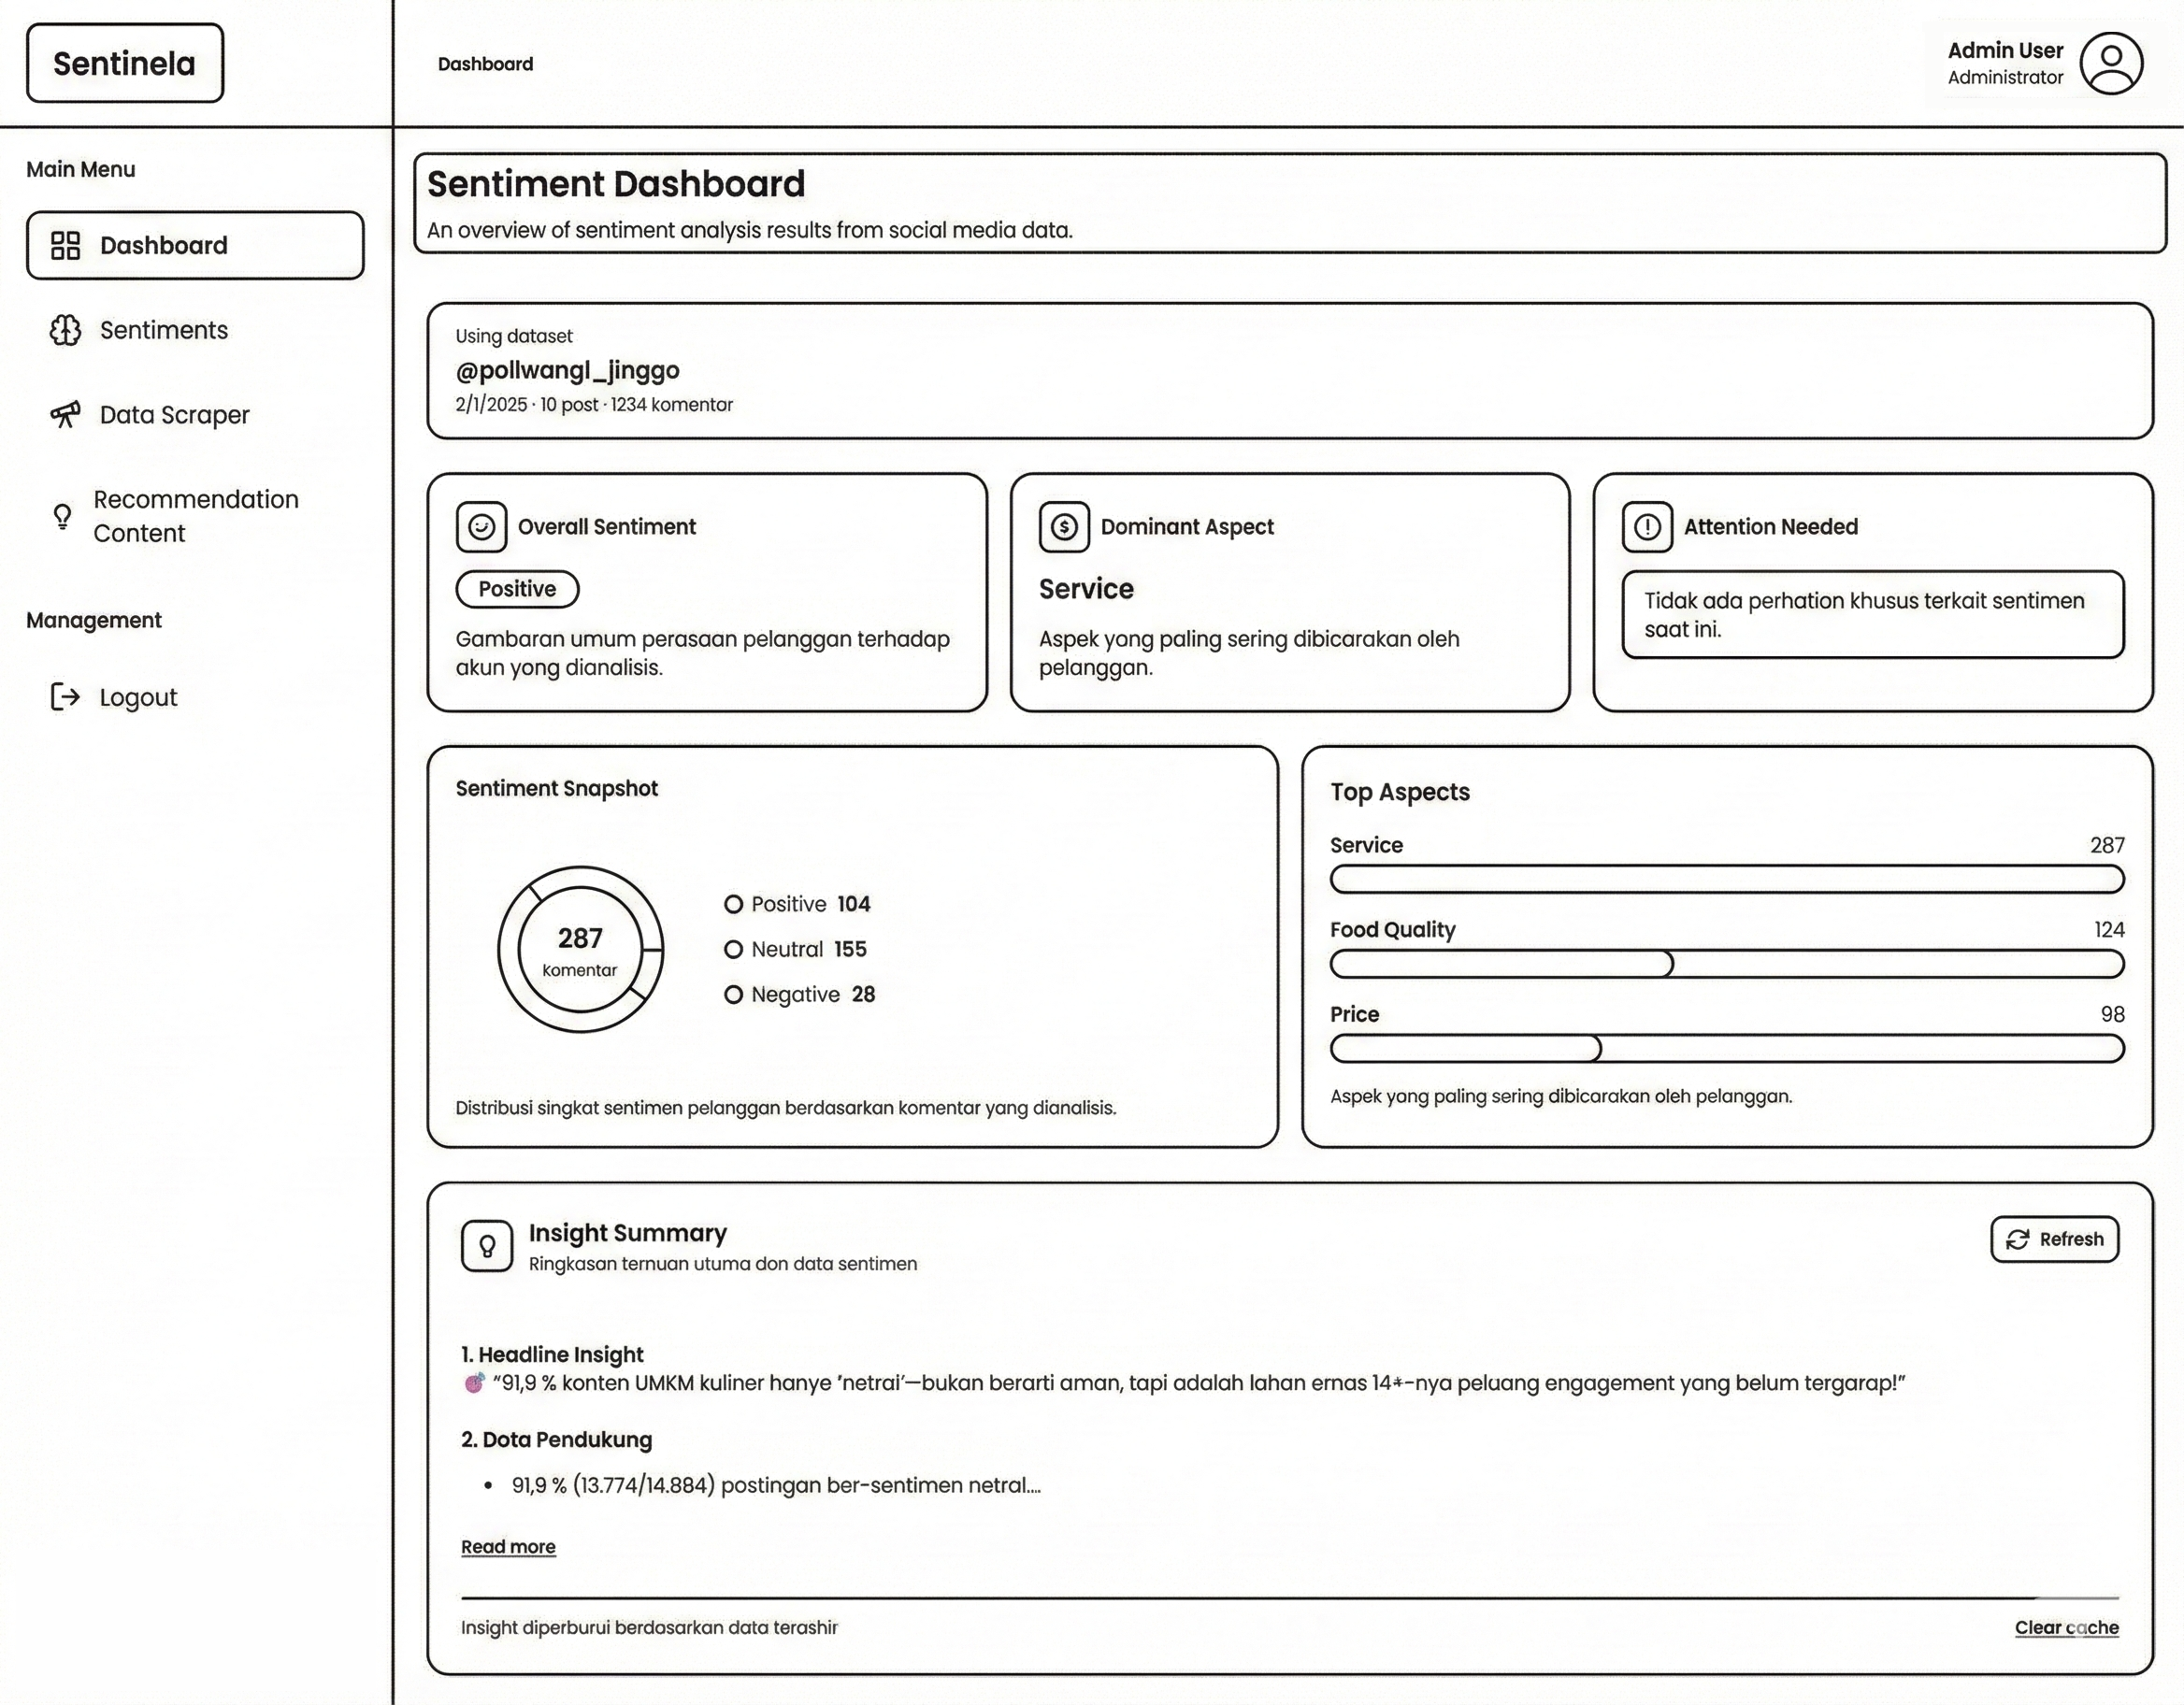
\includegraphics[width=0.6\textwidth]{gambar/dashboard.png}
  \caption{Wireframe Halaman Dashboard}
  \label{fig:dashboard}
\end{figure}

Halaman Dashboard pada Gambar \ref{fig:dashboard} dirancang sebagai halaman utama setelah pengguna berhasil melakukan autentikasi. Halaman ini berfungsi sebagai pusat informasi yang menampilkan ringkasan data dan visualisasi utama dari sistem. Struktur dashboard dirancang untuk memudahkan pengguna dalam memantau kondisi data secara keseluruhan serta mengakses fitur-fitur utama melalui navigasi yang tersedia. Perancangan wireframe ini bertujuan untuk memastikan penyajian informasi yang terstruktur dan mudah dipahami, sehingga pengguna dapat memperoleh gambaran umum hasil analisis secara cepat sebelum melakukan eksplorasi data lebih lanjut.

% wireframe sentiment
\begin{figure}[H]
  \centering
  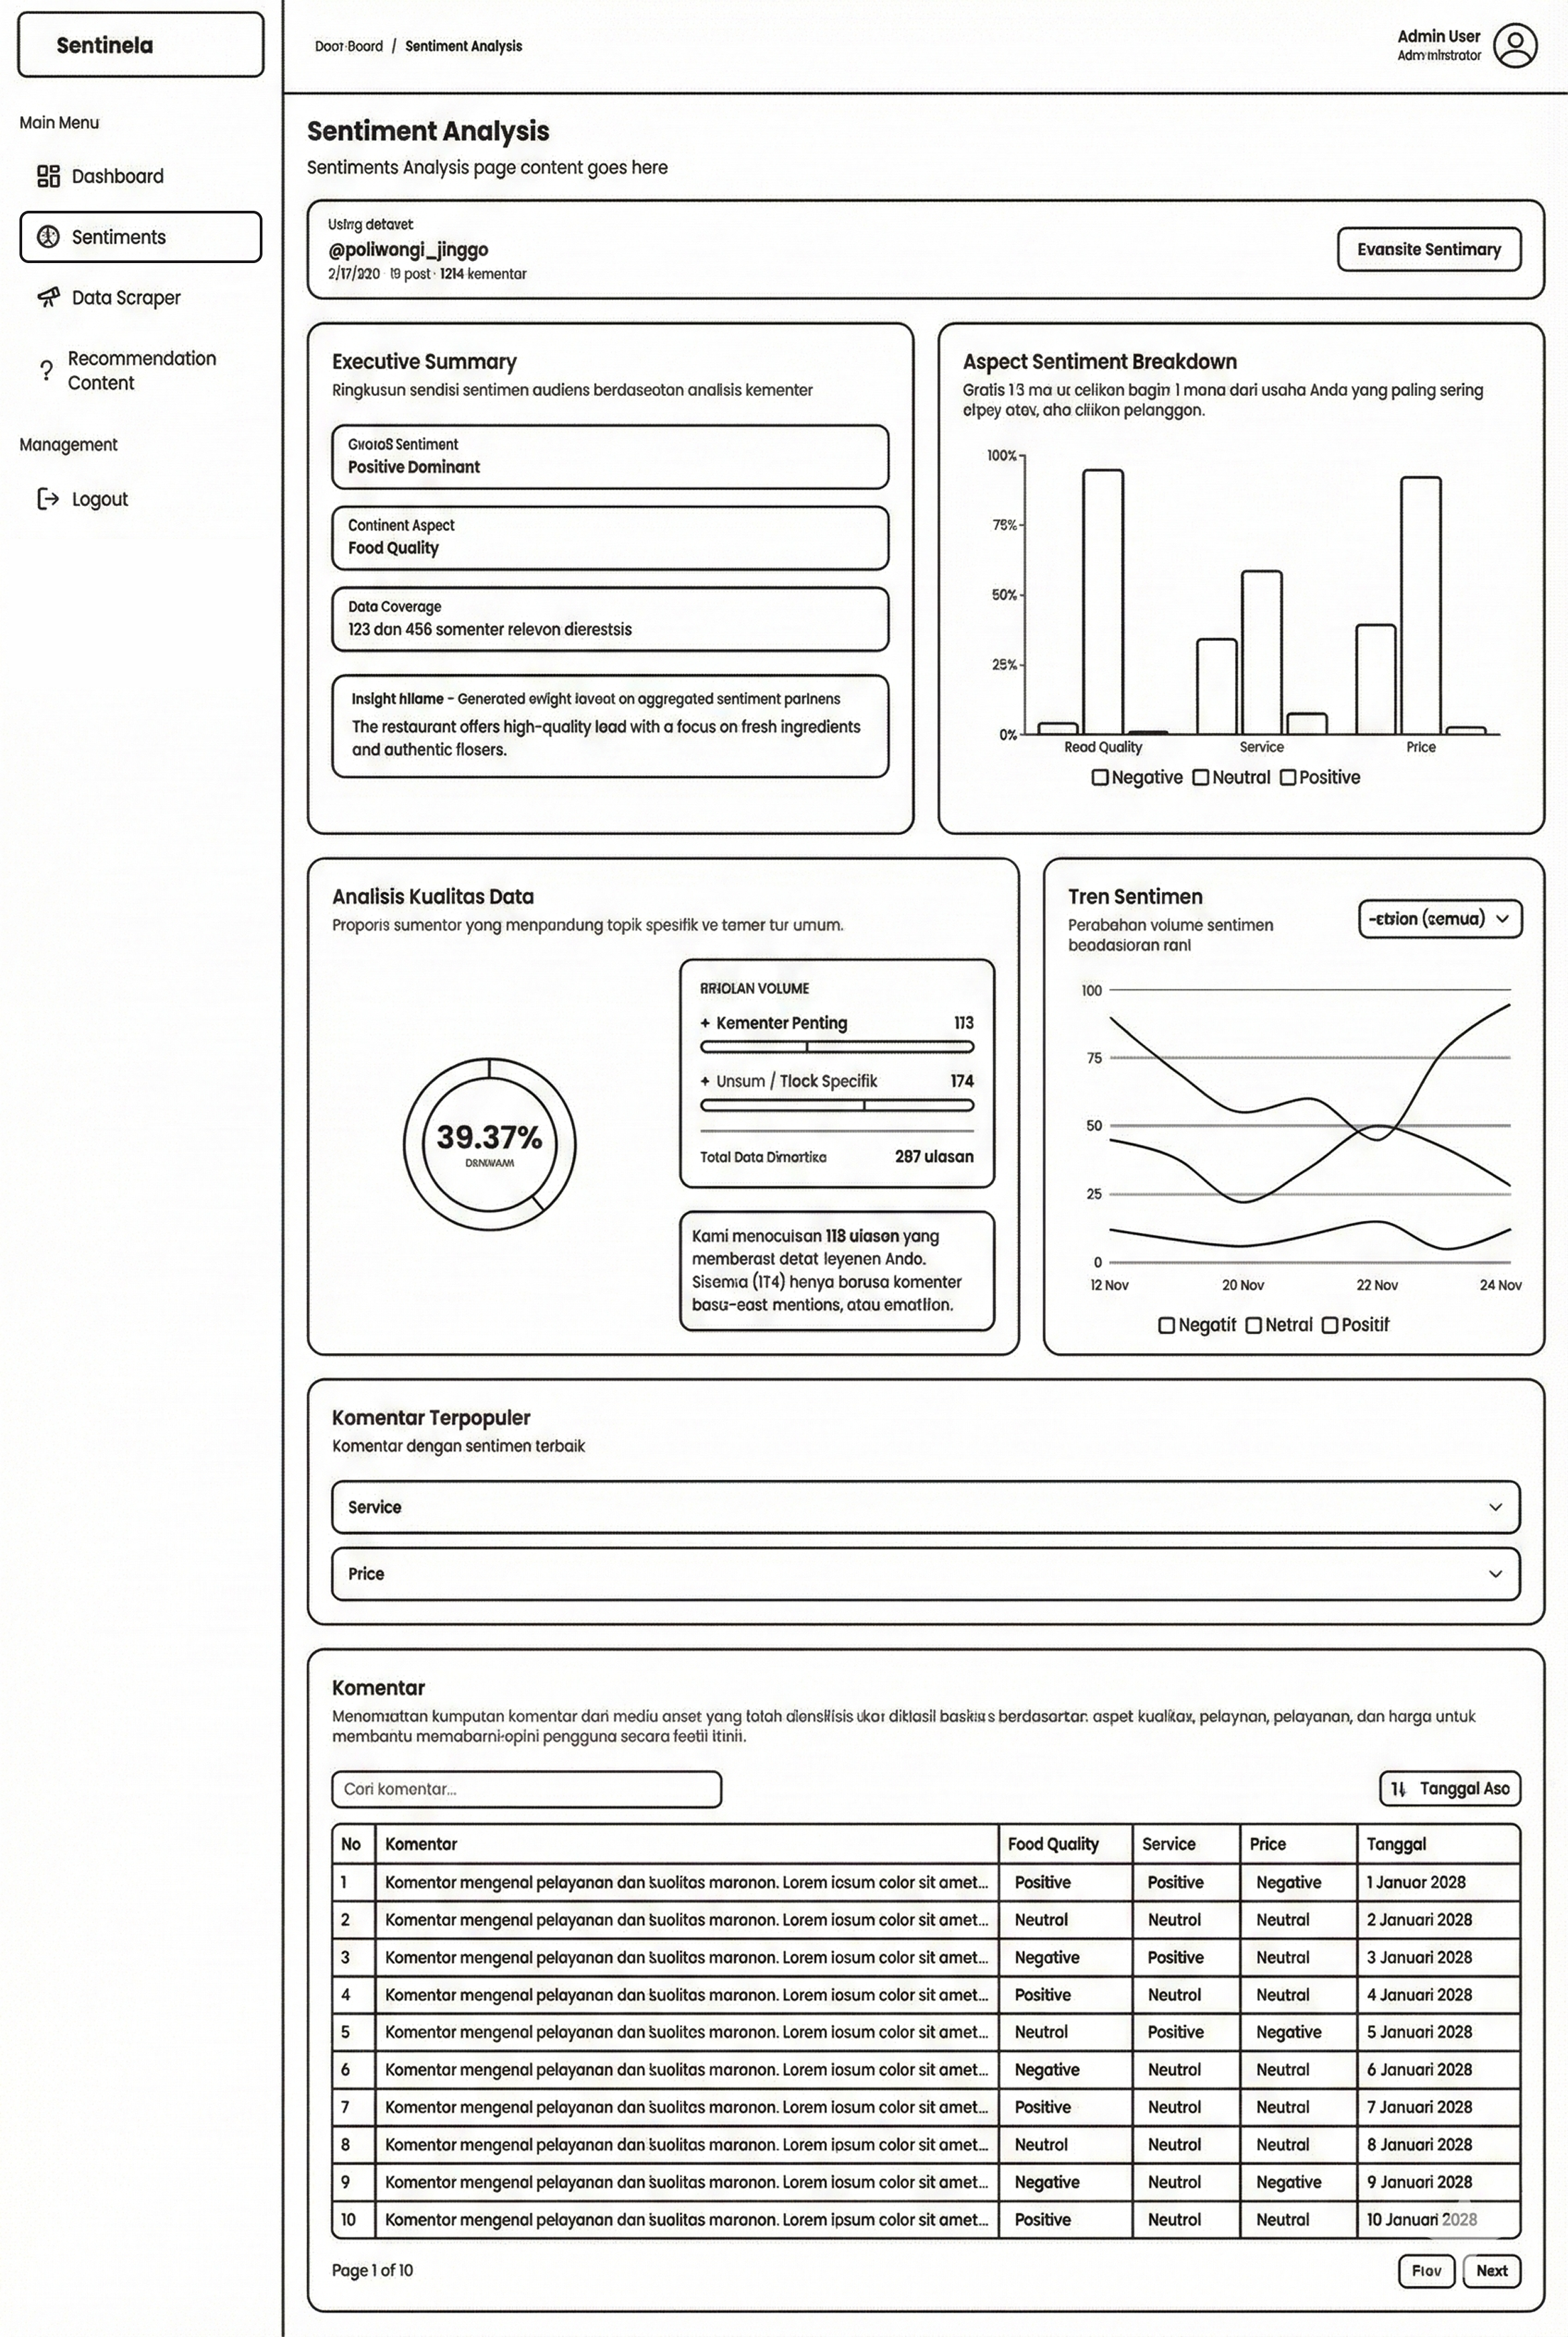
\includegraphics[width=0.6\textwidth]{gambar/sentiment.png}
  \caption{Wireframe Halaman Sentiment}
  \label{fig:sentiment}
\end{figure}

Halaman Sentiment pada Gambar \ref{fig:sentiment} dirancang untuk menampilkan hasil analisis sentimen aspect based sentiment analysis secara lebih rinci dibandingkan halaman dashboard. Halaman ini menyajikan informasi sentimen dalam bentuk visualisasi data yang memudahkan pengguna dalam memahami distribusi dan kecenderungan sentimen. Perancangan struktur halaman difokuskan pada penyajian data yang terorganisasi dan mudah diinterpretasikan, sehingga pengguna dapat melakukan analisis sentimen secara lebih mendalam sesuai dengan kebutuhan informasi yang diinginkan.

% wireframe scraper
\begin{figure}[H]
  \centering
  \includegraphics[width=0.6\textwidth]{gambar/scraper.png}
  \caption{Wireframe Halaman Scraper}
  \label{fig:scraper}
\end{figure}

Halaman Scraper pada Gambar \ref{fig:scraper} dirancang sebagai antarmuka yang memfasilitasi proses pengumpulan dan pemantauan data yang bersumber dari media sosial. Halaman ini menyajikan data hasil proses scraping yang dilakukan pada sisi server, sehingga pengguna dapat mengetahui data yang tersedia dan data yang mana yang akan digunakan oleh sistem pada tahap analisis.

% wireframe recomendation
\begin{figure}[H]
  \centering
  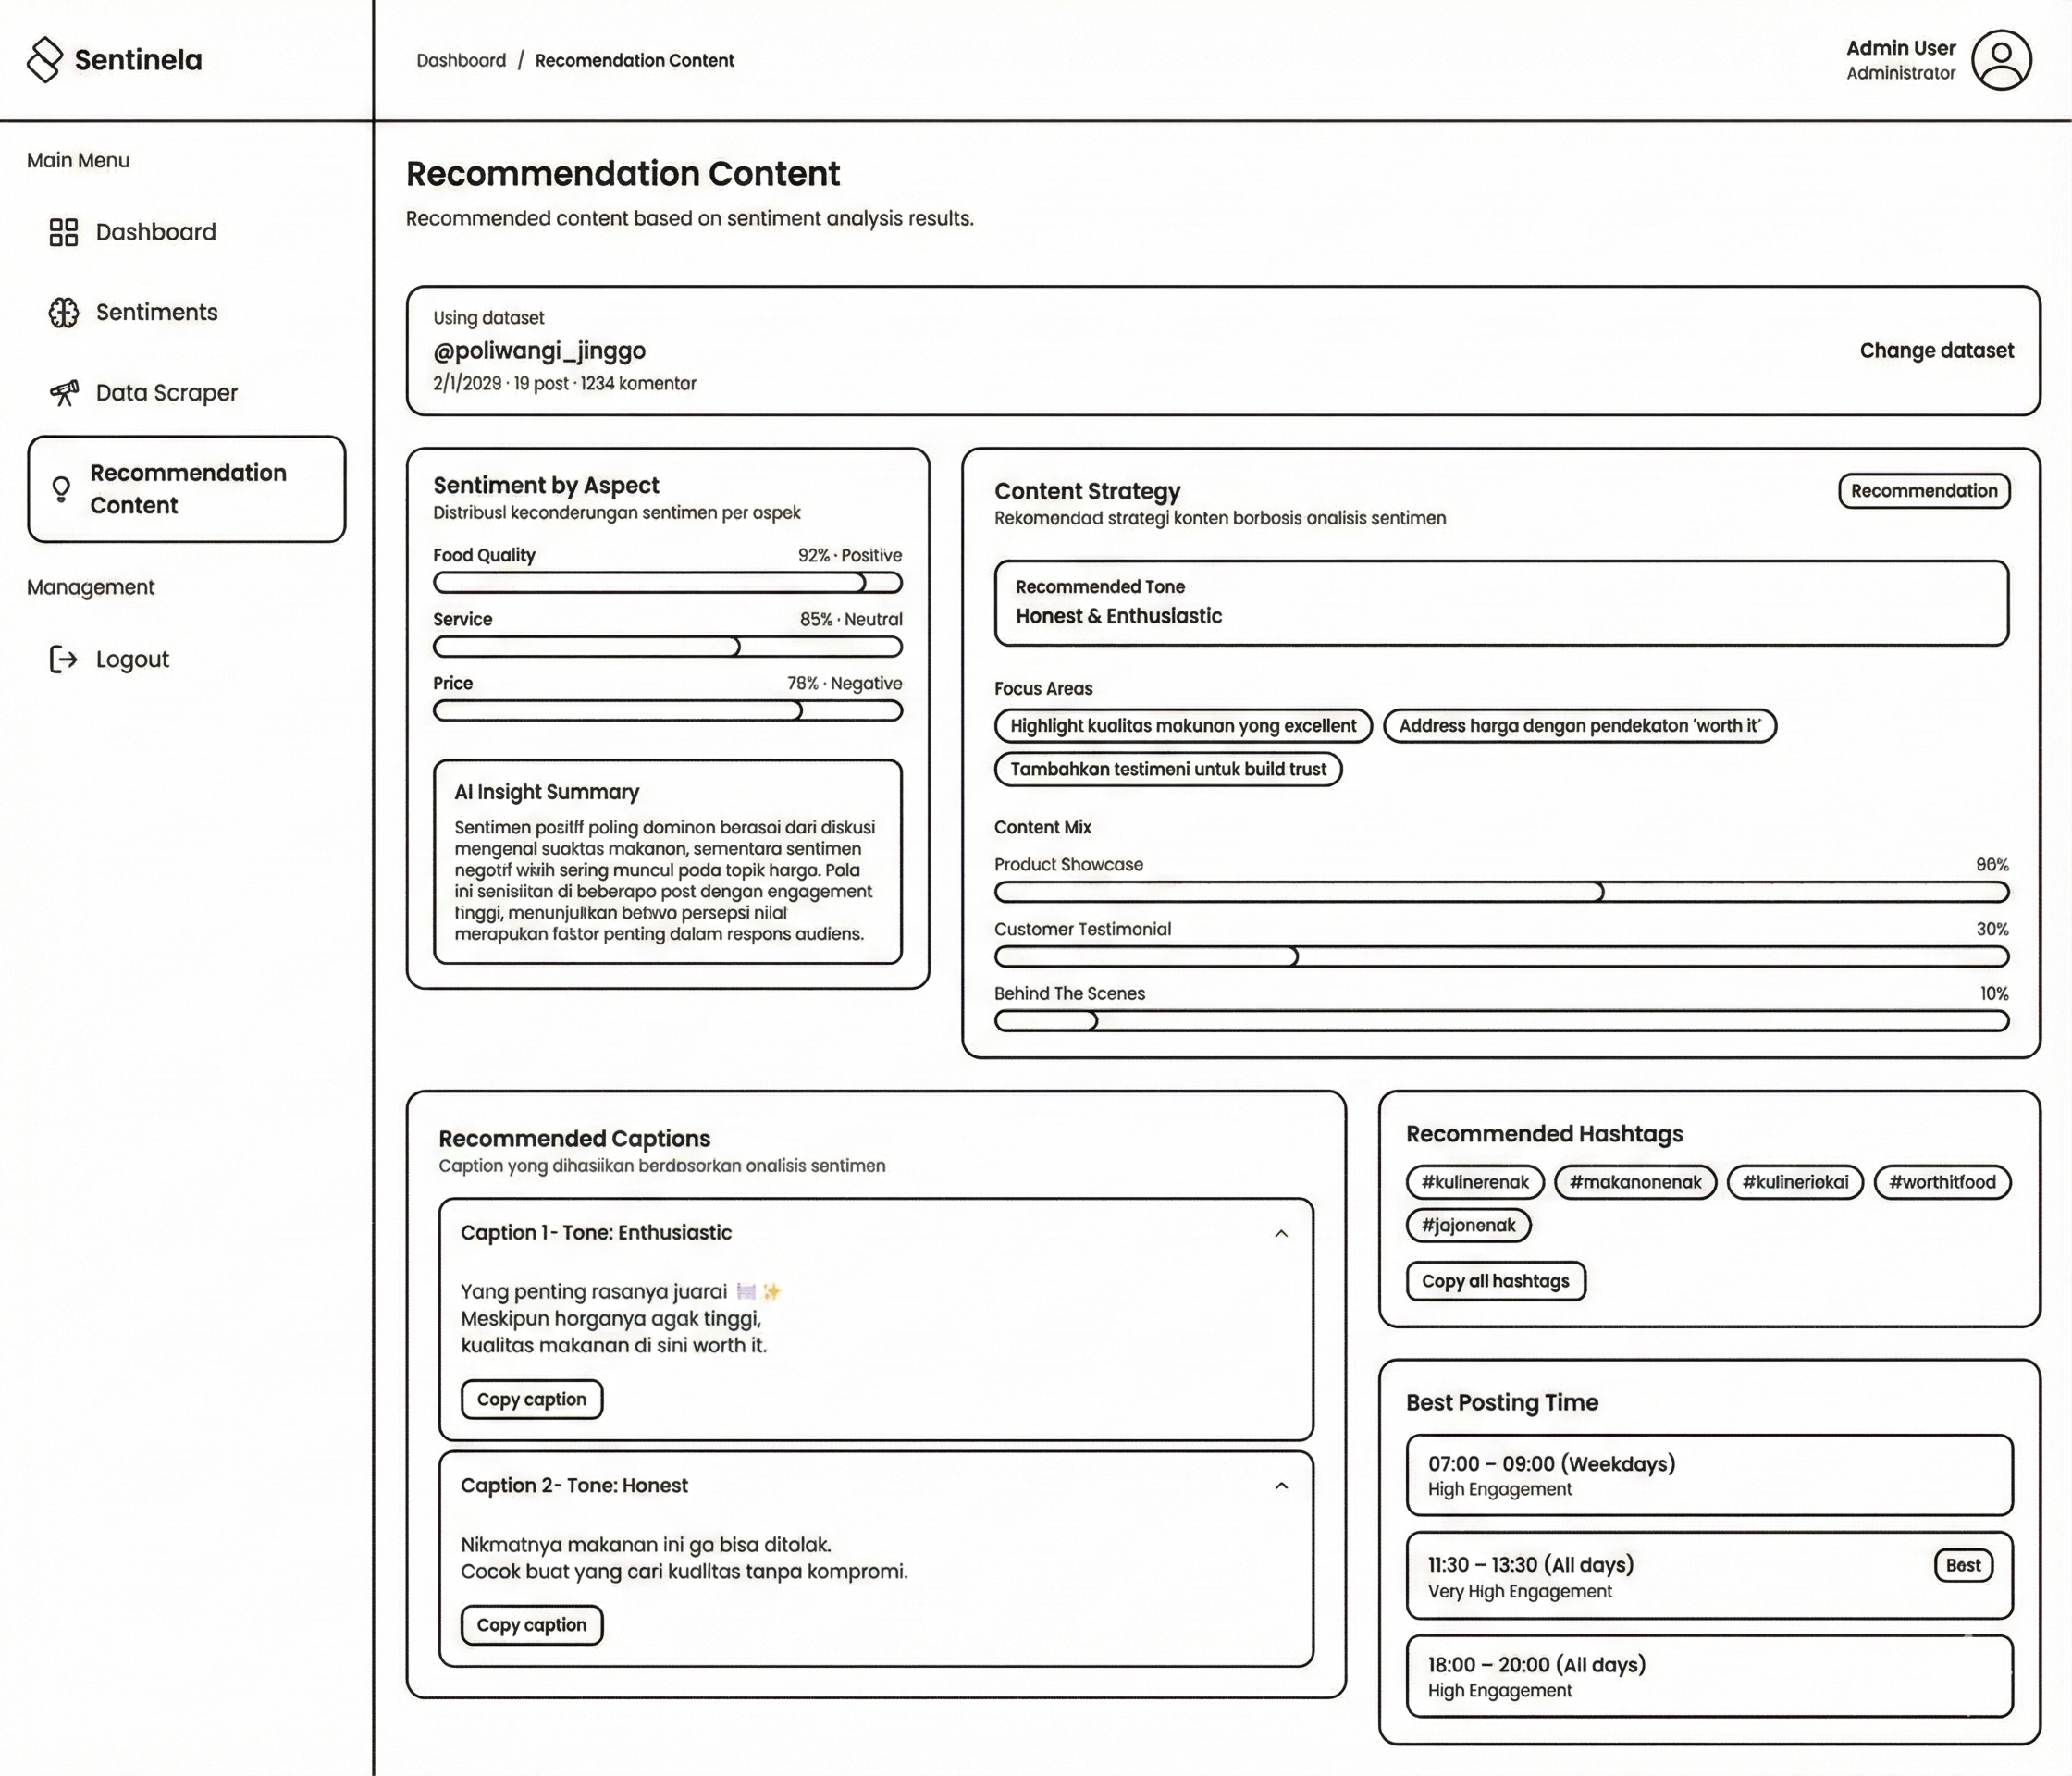
\includegraphics[width=0.6\textwidth]{gambar/recomendation.png}
  \caption{Wireframe Halaman Recomendation}
  \label{fig:recomendation}
\end{figure}

Halaman Recommendation pada Gambar \ref{fig:recomendation} dirancang sebagai antarmuka yang menyajikan rekomendasi berdasarkan hasil analisis sentimen yang telah diproses secara otomatis oleh sistem. Halaman ini menampilkan informasi rekomendasi yang diperoleh dari pengolahan data sentimen, sehingga pengguna dapat memahami insight yang dihasilkan dari data media sosial. Hasil rekomendasi yang ditampilkan pada halaman ini juga disajikan secara lebih detail sebagai bagian dari informasi rekomendasi utama. Halaman ini bertujuan untuk memudahkan pengguna dalam mengakses rekomendasi dan memahami hasil analisis sentimen secara terstruktur.

\section{Metode Pengujian dan Evaluasi Sistem}

\subsection{Metode Pengujian}

Metode pengujian yang digunakan dalam penelitian ini mengacu pada konsep black-box testing yang telah dijelaskan pada Bab II, dengan pendekatan scenario-based testing. Pengujian dilakukan dengan mengamati perilaku sistem berdasarkan skenario penggunaan tanpa memperhatikan struktur internal kode program. Pendekatan ini menempatkan sistem sebagai sebuah kesatuan yang diuji dari sudut pandang pengguna, sehingga pengujian difokuskan pada kesesuaian fungsi dan respons sistem terhadap alur penggunaan yang dirancang.

Pemilihan pendekatan scenario-based testing didasarkan pada karakteristik sistem yang dikembangkan, yaitu dashboard analitik yang bersifat data-driven dan mengandalkan interaksi antar-komponen antarmuka. Oleh karena itu, pengujian diarahkan pada evaluasi perilaku sistem dalam menampilkan data, menjaga konsistensi informasi, serta merespons pembaruan data sesuai dengan kondisi yang terjadi.

Ruang lingkup pengujian pada penelitian ini difokuskan pada perilaku sistem frontend, khususnya pada pengelolaan data melalui Client Data Layer dan penyajian data pada antarmuka pengguna. Pengujian tidak mencakup evaluasi terhadap algoritma analisis sentimen maupun proses pengolahan data pada sisi backend.

\subsection{Skenario dan Objek Pengujian}

Skenario pengujian disusun berdasarkan fitur utama sistem dan merepresentasikan alur penggunaan dari sudut pandang pengguna. Setiap skenario dirancang untuk mengevaluasi perilaku sistem frontend dalam merespons interaksi pengguna serta memastikan kesesuaian fungsi sistem dengan rancangan yang telah ditetapkan. Skenario pengujian dalam penelitian ini terdiri atas beberapa pengujian sebagai berikut:

\begin{packed_enum}

\item Landing Page

\begin{table}[H]
\centering
\caption{Skenario Pengujian Landing Page}
\label{tab:pengujian-landing-page}
\renewcommand{\arraystretch}{1.4}

\begin{tabular}{|c|p{3cm}|p{4cm}|p{2cm}|p{5cm}|}
\hline
\textbf{ID} &
\textbf{Fitur} &
\textbf{Skenario Pengujian} &
\textbf{Data Uji} &
\textbf{Hasil yang Diharapkan} \\ \hline

TC-01 &
Landing Page &
Pengguna membuka aplikasi tanpa melakukan proses login &
-- &
Halaman landing tampil dengan informasi sistem serta navigasi menuju halaman login dan registrasi. \\ \hline

\end{tabular}
\end{table}


\item Login

\begin{table}[H]
\centering
\caption{Skenario Pengujian Halaman Login}
\label{tab:login-testing}
\begin{tabular}{|c|p{3cm}|p{5cm}|p{3.5cm}|p{4.5cm}|}
\hline
\textbf{ID} & \textbf{Fitur} & \textbf{Skenario Pengujian} & \textbf{Data Uji} & \textbf{Hasil yang Diharapkan} \\
\hline
TC-LG-01 & Login & Pengguna melakukan login dengan kredensial yang valid & Email dan kata sandi valid & Sistem berhasil mengautentikasi pengguna dan mengarahkan ke halaman dashboard \\
\hline
TC-LG-02 & Login & Pengguna melakukan login dengan kata sandi yang salah & Email valid, kata sandi salah & Sistem menampilkan pesan kesalahan dan tetap berada di halaman login \\
\hline
TC-LG-03 & Login & Pengguna melakukan login dengan email yang tidak terdaftar & Email tidak terdaftar & Sistem menampilkan pesan bahwa akun tidak ditemukan \\
\hline
TC-LG-04 & Login & Pengguna mengirimkan formulir login dengan field kosong & Email atau kata sandi kosong & Sistem menampilkan validasi bahwa data login harus diisi \\
\hline
TC-LG-05 & Login & Pengguna berhasil login setelah sebelumnya gagal login & Kredensial valid & Sistem menerima kredensial dan mengarahkan pengguna ke halaman dashboard \\
\hline
\end{tabular}
\end{table}


\item Register

\begin{table}[H]
\centering
\caption{Skenario Pengujian Halaman Register}
\label{tab:register-testing}
\begin{tabular}{|c|p{3cm}|p{5cm}|p{3.5cm}|p{4.5cm}|}
\hline
\textbf{ID} & \textbf{Fitur} & \textbf{Skenario Pengujian} & \textbf{Data Uji} & \textbf{Hasil yang Diharapkan} \\
\hline
TC-RG-01 & Register & Pengguna melakukan pendaftaran dengan data yang valid & Data registrasi lengkap dan valid & Sistem berhasil menyimpan data pengguna dan akun dapat digunakan untuk login \\
\hline
TC-RG-02 & Register & Pengguna melakukan pendaftaran dengan data tidak lengkap & Salah satu atau beberapa field kosong & Sistem menampilkan pesan validasi bahwa data registrasi harus diisi lengkap \\
\hline
TC-RG-03 & Register & Pengguna melakukan pendaftaran dengan format data tidak sesuai & Format email tidak valid & Sistem menampilkan pesan kesalahan format data \\
\hline
TC-RG-04 & Register & Pengguna mendaftarkan akun dengan email yang sudah terdaftar & Email sudah terdaftar & Sistem menampilkan pesan bahwa akun sudah terdaftar \\
\hline
TC-RG-05 & Register & Pengguna mengirimkan ulang data registrasi setelah terjadi kesalahan & Data registrasi valid & Sistem menerima data dan proses registrasi berhasil \\
\hline
\end{tabular}
\end{table}



\item Dashboard

\begin{table}[H]
\centering
\caption{Skenario Pengujian Halaman Dashboard}
\label{tab:dashboard-testing}
\begin{tabular}{|c|p{3cm}|p{5cm}|p{3.5cm}|p{4.5cm}|}
\hline
\textbf{ID} & \textbf{Fitur} & \textbf{Skenario Pengujian} & \textbf{Data Uji} & \textbf{Hasil yang Diharapkan} \\
\hline
TC-DB-01 & Dashboard & Pengguna membuka halaman dashboard setelah login & Data dashboard tersedia & Sistem menampilkan ringkasan data dan visualisasi utama pada dashboard \\
\hline
TC-DB-02 & Dashboard & Pengguna membuka dashboard dengan data belum tersedia & Data belum tersedia & Sistem menampilkan indikator pemuatan atau pesan informasi \\
\hline
TC-DB-03 & Dashboard & Pengguna melakukan navigasi ke menu lain dan kembali ke dashboard & -- & Sistem menampilkan data dashboard secara konsisten tanpa kehilangan data \\
\hline
TC-DB-04 & Dashboard & Pembaruan data dashboard dari server & Data diperbarui & Sistem memperbarui tampilan dashboard sesuai data terbaru \\
\hline
TC-DB-05 & Dashboard & Beberapa komponen menggunakan sumber data yang sama & Data yang sama digunakan & Sistem menampilkan data yang konsisten pada seluruh komponen dashboard \\
\hline
\end{tabular}
\end{table}

\item Sentiment

\begin{table}[H]
\centering
\caption{Skenario Pengujian Halaman Dashboard Sentiment}
\label{tab:sentiment-testing}
\begin{tabular}{|c|p{3cm}|p{5cm}|p{3.5cm}|p{4.5cm}|}
\hline
\textbf{ID} & \textbf{Fitur} & \textbf{Skenario Pengujian} & \textbf{Data Uji} & \textbf{Hasil yang Diharapkan} \\
\hline
TC-ST-01 & Dashboard Sentiment & Pengguna membuka halaman dashboard sentiment & Data sentimen tersedia & Sistem menampilkan visualisasi dan ringkasan hasil analisis sentimen \\
\hline
TC-ST-02 & Dashboard Sentiment & Pengguna membuka halaman sentiment dengan data belum tersedia & Data sentimen belum tersedia & Sistem menampilkan indikator pemuatan atau pesan informasi \\
\hline
TC-ST-03 & Dashboard Sentiment & Pembaruan data sentimen dari server & Data sentimen diperbarui & Sistem memperbarui visualisasi sesuai data sentimen terbaru \\
\hline
TC-ST-04 & Dashboard Sentiment & Navigasi ke halaman lain dan kembali ke dashboard sentiment & -- & Sistem menampilkan data sentimen secara konsisten tanpa kehilangan data \\
\hline
TC-ST-05 & Dashboard Sentiment & Beberapa komponen menampilkan data sentimen yang sama & Data sentimen yang sama digunakan & Sistem menampilkan data yang konsisten pada seluruh komponen visualisasi \\
\hline
\end{tabular}
\end{table}

\item Recommendation

\begin{table}[H]
\centering
\caption{Skenario Pengujian Halaman Dashboard Rekomendasi Konten}
\label{tab:recommendation-testing}
\begin{tabular}{|c|p{3cm}|p{5cm}|p{3.5cm}|p{4.5cm}|}
\hline
\textbf{ID} & \textbf{Fitur} & \textbf{Skenario Pengujian} & \textbf{Data Uji} & \textbf{Hasil yang Diharapkan} \\
\hline
TC-RC-01 & Dashboard Rekomendasi & Pengguna membuka halaman dashboard rekomendasi konten & Data rekomendasi tersedia & Sistem menampilkan daftar rekomendasi berdasarkan hasil analisis sentimen \\
\hline
TC-RC-02 & Dashboard Rekomendasi & Pengguna membuka halaman rekomendasi dengan data belum tersedia & Data rekomendasi belum tersedia & Sistem menampilkan indikator pemuatan atau pesan informasi \\
\hline
TC-RC-03 & Dashboard Rekomendasi & Pembaruan data rekomendasi dari server & Data rekomendasi diperbarui & Sistem memperbarui tampilan rekomendasi sesuai data terbaru \\
\hline
TC-RC-04 & Dashboard Rekomendasi & Navigasi ke halaman lain dan kembali ke dashboard rekomendasi & -- & Sistem menampilkan data rekomendasi secara konsisten \\
\hline
TC-RC-05 & Dashboard Rekomendasi & Konsistensi rekomendasi dengan data sentimen & Data sentimen terkait berubah & Rekomendasi konten menyesuaikan perubahan data sentimen \\
\hline
\end{tabular}
\end{table}


\item Scraper

\begin{table}[H]
\centering
\caption{Skenario Pengujian Halaman Data Scraper}
\label{tab:scraper-testing}
\begin{tabular}{|c|p{3cm}|p{5cm}|p{3.5cm}|p{4.5cm}|}
\hline
\textbf{ID} & \textbf{Fitur} & \textbf{Skenario Pengujian} & \textbf{Data Uji} & \textbf{Hasil yang Diharapkan} \\
\hline
TC-SC-01 & Data Scraper & Pengguna membuka halaman data scraper & Data hasil scraping tersedia & Sistem menampilkan daftar data hasil scraping yang diperoleh dari server \\
\hline
TC-SC-02 & Data Scraper & Pengguna membuka halaman scraper dengan data belum tersedia & Data belum tersedia & Sistem menampilkan indikator pemuatan atau pesan informasi \\
\hline
TC-SC-03 & Data Scraper & Pengguna memilih data untuk dianalisis & Dataset tertentu dipilih & Sistem menandai data terpilih untuk digunakan pada proses analisis \\
\hline
TC-SC-04 & Data Scraper & Navigasi ke halaman lain dan kembali ke data scraper & -- & Sistem menampilkan data scraper secara konsisten tanpa kehilangan data \\
\hline
\end{tabular}
\end{table}


\item Chatbot

\begin{table}[H]
\centering
\caption{Skenario Pengujian Chatbot}
\label{tab:chatbot-testing}
\begin{tabular}{|c|p{3cm}|p{5cm}|p{3.5cm}|p{4.5cm}|}
\hline
\textbf{ID} & \textbf{Fitur} & \textbf{Skenario Pengujian} & \textbf{Data Uji} & \textbf{Hasil yang Diharapkan} \\
\hline
TC-CB-01 & Chatbot & Pengguna membuka fitur chatbot & -- & Sistem menampilkan antarmuka chatbot dan siap menerima input pengguna \\
\hline
TC-CB-02 & Chatbot & Pengguna mengirimkan pertanyaan melalui chatbot & Pertanyaan teks valid & Sistem menampilkan respons chatbot sesuai dengan pertanyaan yang diberikan \\
\hline
TC-CB-03 & Chatbot & Pengguna mengirimkan input kosong & Input kosong & Sistem menampilkan pesan validasi atau respons bahwa input tidak valid \\
\hline
TC-CB-04 & Chatbot & Pengguna mengirimkan pertanyaan di luar konteks sistem & Pertanyaan tidak relevan & Sistem tetap memberikan respons atau pesan informasi yang sesuai \\
\hline
TC-CB-05 & Chatbot & Pengguna melakukan interaksi berulang dengan chatbot & Beberapa pertanyaan berurutan & Sistem mampu menampilkan respons secara konsisten pada setiap interaksi \\
\hline
\end{tabular}
\end{table}


\item Logout

\begin{table}[H]
\centering
\caption{Skenario Pengujian Logout}
\label{tab:logout-testing}
\begin{tabular}{|c|p{3cm}|p{5cm}|p{3.5cm}|p{4.5cm}|}
\hline
\textbf{ID} & \textbf{Fitur} & \textbf{Skenario Pengujian} & \textbf{Data Uji} & \textbf{Hasil yang Diharapkan} \\
\hline
TC-LO-01 & Logout & Pengguna melakukan logout dari sistem & -- & Sistem mengakhiri sesi pengguna dan mengarahkan ke halaman login \\
\hline
TC-LO-02 & Logout & Pengguna mencoba mengakses halaman dashboard setelah logout & -- & Sistem menolak akses dan mengarahkan kembali ke halaman login \\
\hline
TC-LO-03 & Logout & Pengguna menutup sesi dan membuka ulang aplikasi & -- & Sistem meminta pengguna untuk login kembali \\
\hline
\end{tabular}
\end{table}


\end{packed_enum}


\subsection{Teknik Evaluasi}

Teknik evaluasi pada penelitian ini dilakukan untuk menilai kesesuaian perilaku sistem frontend terhadap rancangan arsitektur dan Client Data Layer yang telah ditetapkan. Evaluasi dilakukan dengan pendekatan kualitatif-deskriptif, yaitu melalui observasi terhadap perilaku sistem selama proses pengujian berlangsung tanpa melibatkan pengukuran numerik performa secara detail. Pendekatan ini dipilih karena fokus penelitian diarahkan pada perilaku pengelolaan data dan konsistensi tampilan sistem, bukan pada pengujian efisiensi algoritma atau kinerja backend.

Sumber data evaluasi diperoleh dari hasil observasi terhadap tampilan dashboard serta perilaku pengelolaan data pada sisi frontend. Observasi dilakukan terhadap bagaimana data ditampilkan pada berbagai komponen antarmuka, bagaimana sistem merespons pembaruan data, serta bagaimana konsistensi data terjaga ketika komponen yang berbeda menggunakan sumber data yang sama. Selain itu, evaluasi juga dilakukan dengan mengamati log permintaan data untuk memastikan bahwa mekanisme pengelolaan data berjalan sesuai dengan rancangan.

Sebagai alat bantu evaluasi, penelitian ini memanfaatkan fitur observasi yang disediakan oleh TanStack Query Devtools. Alat bantu ini digunakan untuk memantau status pengambilan data, mekanisme penyimpanan sementara (caching), serta proses sinkronisasi data antar-komponen selama skenario pengujian dijalankan. Penggunaan alat bantu ini bertujuan untuk mendukung proses observasi perilaku sistem secara lebih terstruktur, tanpa bergantung pada detail implementasi kode program.

Indikator evaluasi dalam penelitian ini meliputi beberapa aspek utama, yaitu konsistensi data antar-komponen antarmuka, perilaku mekanisme caching dalam mengendalikan permintaan data berulang, serta kemampuan sistem dalam menyinkronkan pembaruan data sesuai dengan kondisi yang terjadi pada sisi backend. Selain itu, evaluasi juga dilakukan untuk memastikan bahwa perilaku sistem frontend telah sesuai dengan perancangan Client Data Layer dan arsitektur frontend yang direncanakan pada tahap perancangan sistem.

Sistem frontend dinilai berhasil apabila seluruh indikator evaluasi tersebut terpenuhi dan tidak ditemukan ketidaksesuaian perilaku sistem selama skenario pengujian dijalankan.







